After nearly a decade of absence, non-linear optics finally appears again this year, albeit with a new perspective on wave generation!
\begin{parts}
	\part Explanation of how a non-linear response in a medium gives rise to second harmonic generation.
	
	We begin by inspecting the definition of second-order susceptibility $\chi^{(2)}$ in a non-linear crystal:
	\begin{equation}
		P^{(2)}_{i} = \epsilon_0 \chi^{(2)}_{ijk} E_j E_k
		\label{eqn:q2-second-susceptibility}
	\end{equation}
	
	The interaction between $E_j$ and $E_k$ to produce $P_i$ is called wave-mixing.
	In the case where both terms possess the same frequency, \eqref{eqn:q2-second-susceptibility} tells us that components with frequencies $\omega\pm\omega$ are produced -- thereby producing a second harmonics and an optically-rectified field.
	
	Phase difference $\Delta k$ is given as:
	\begin{equation*}
		\Delta k = k_3 - 2k_1
	\end{equation*}
	
	\part Bookwork -- this should be very familiar for those who had done parametric wave mixing for their projects.
	
	Starting from the given $\partial A_3 / \partial x$, we invoke the non-depleting-pump approximation where $A_1$ is constant, thus:
	\begin{align}
		\frac{\partial A_3}{\partial x} &= \beta A_1^2 \exp(-i\Delta kx) \notag \\
		\Rightarrow A_3 (x) - A_3 (0) &= \beta A_1^2 \frac{\exp(-i\Delta kx) - \exp(0)}{-i\Delta k} \notag \\
		A_3 (x)&= \beta A_1^2 \frac{\exp(-i\Delta kx) - 1}{-i\Delta k} \notag \\
		&= \beta A_1^2 \exp\left(\frac{-i\Delta k x}{2}\right) \frac{\sin\left(\frac{\Delta kx}{2}\right)}{i\Delta k} \notag \\
		&= 2\beta A_1^2 \exp\left(\frac{-i\Delta k x}{2}\right) x\, \textnormal{sinc}\left(\frac{\Delta kx}{2}\right)
		\label{eqn:q2-a3-x}
	\end{align}
	where $A_3 (0)$ is assumed to be null.
	
	Therefore the intensity of the second harmonics is:
	\begin{align*}
		I_3 (x) &\propto \left|A_3\right|^2 \\
		&\propto 4\beta^2 \left|A_1^2\right|^2 x^2 \textnormal{sinc}^2\left(\frac{\Delta kx}{2}\right) \\
		&\propto I_1^2 \, x^2 \, \textnormal{sinc}^2\left(\frac{\Delta kx}{2}\right)
	\end{align*}
	
	\newpage
	Now onto the sketches:
	\begin{subparts}
		\subpart For $\Delta k = 0$, the sinc term vanishes, hence we have $I_3 (x) \propto x^2$:
		\begin{figure}[H]
			\centering
			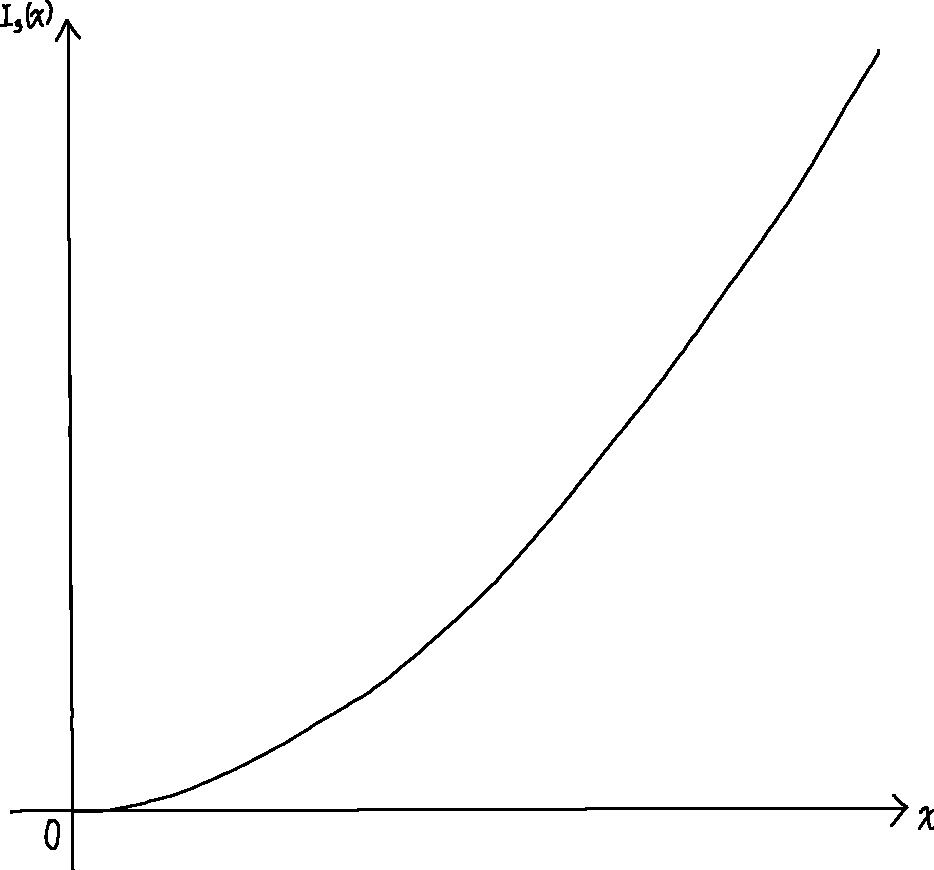
\includegraphics[width=.75\linewidth]{q2-delta-k-zero}
		\end{figure}
		
		\subpart For $\Delta k \neq 0$, the sinc term does not vanish and thus $I_3 (x) \propto \sin^2(\Delta kx/2)$:
		\begin{figure}[H]
			\centering
			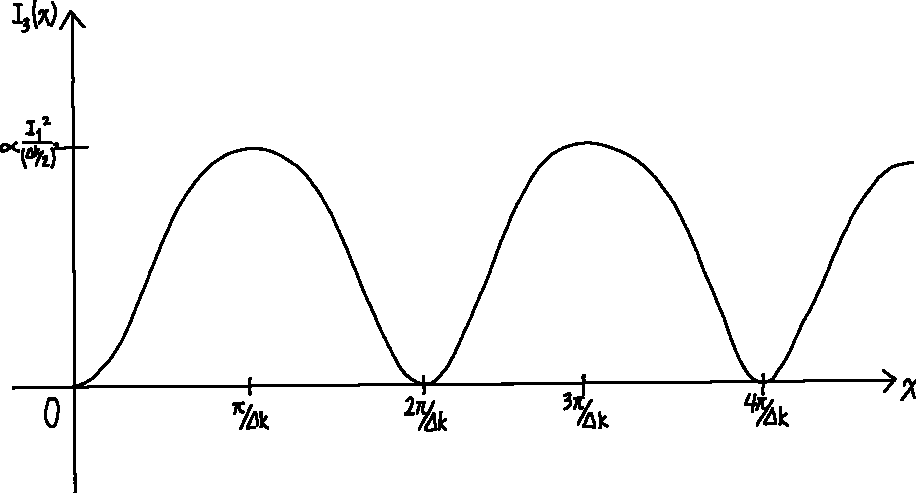
\includegraphics[width=.9\linewidth]{q2-delta-k-nonzero}
		\end{figure}
	\end{subparts}
	The difference between these two cases may be illustrated by the phasor diagram below:
	\begin{figure}[H]
		\centering
		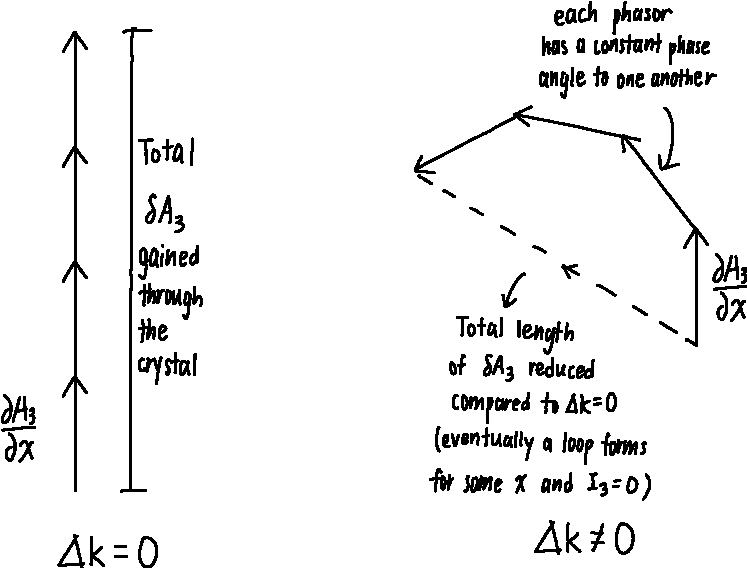
\includegraphics[width=.8\linewidth]{q2-phasor}
	\end{figure}
	In the case of $\Delta k = 0$, the phasors in each $\mathrm{d}x$ step are perfectly aligned to one another, thereby maximising the growth in $A_3$ as we integrate along $x$.
	
	However for $\Delta k \neq 0$, the phasors in each $\mathrm{d}x$ step would be at an angle to one another, thereby causing an oscillatory behaviour where the beam growth is stunted.
	
	Phase-matching is thus a technique by which the condition $\Delta k = 0$ is achieved.
	In the optical regime, we may align the optic axis of an uniaxial crystal at an angle $\theta$ to the incoming wavevector to vary the refractive index $n(\theta)$, thereby adjusting the resulting wavevector $k=nk_0$ where $k_0$ is the wavevector in vacuum.
	
	The relationship between $n(\theta)$ and $\theta$ may be illustrated by the indicatrix below (only a quadrant is drawn for simplicity):
	\begin{equation*}
		\frac{1}{n^2(\theta)} = \frac{\sin^2 \theta}{n_o^2} + \frac{\cos^2 \theta}{n_e^2}
	\end{equation*}
	\begin{figure}[H]
		\centering
		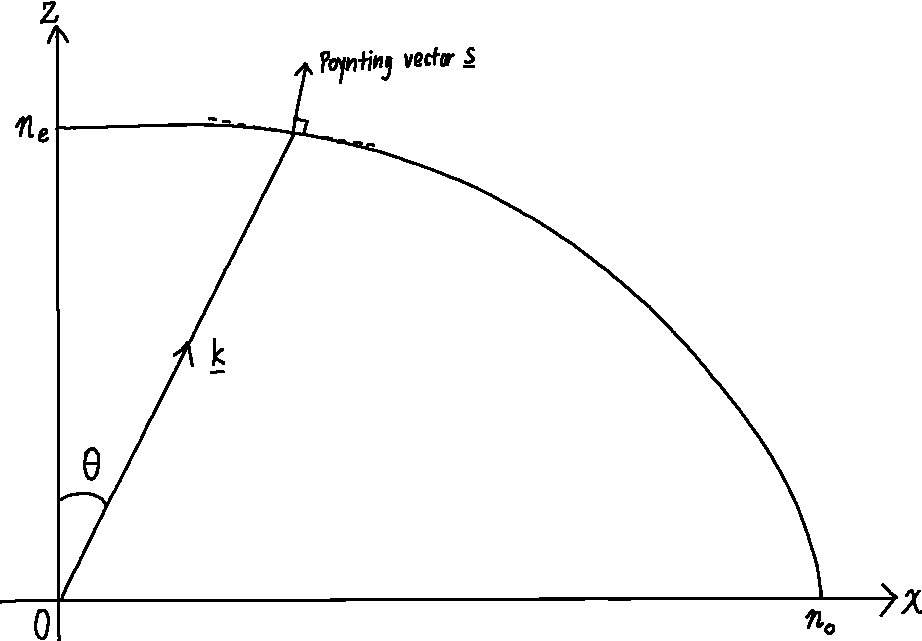
\includegraphics[width=.7\linewidth]{q2-indicatrix}
	\end{figure}
	
	\part The wording here can be rather confusing -- the reversal of crystal axes means the inversion of the sign in $d_{ij}$!
	
	Also take note that the setup here is different from the birefringent case\footnote{In the phasor picture, we are essentially changing the direction of the rotation for every $L_p$ so that the phasors wiggle around the net gain -- this article from RP Photonics has a pretty neat explanation: \url{https://www.rp-photonics.com/quasi_phase_matching.html}}: here both the second harmonics and the pump have the same polarisation, thus the $\beta$ factor differs -- I shall write $\beta_\textnormal{pole} \propto d_{33}$ in the poled crystal case and $\beta_\textnormal{uni} \propto d_{31}$ in the uniform crystal case.
	\begin{figure}[H]
		\centering
		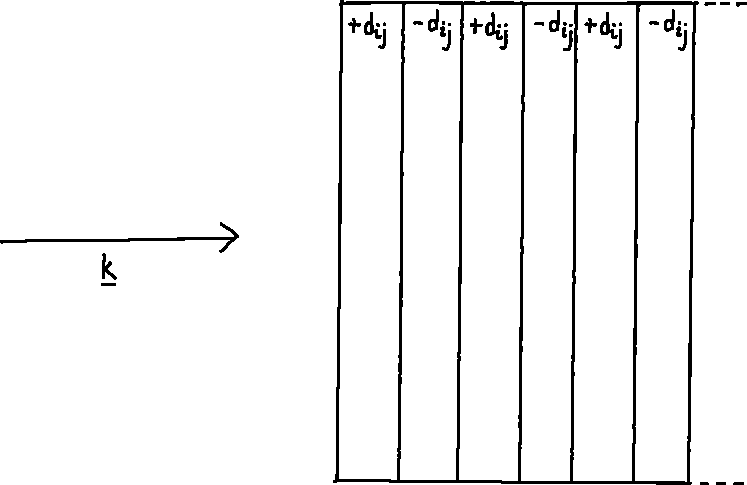
\includegraphics[width=.85\linewidth]{q2-poled-crystal}
	\end{figure}
	
	As suggested by the sketch of $I_3$ against $x$ above, the optimal zone length $L_p$ should be the value of $x$ at which $A_3$ is maximised:
	\begin{gather}
		\sin \left(\frac{\Delta kx}{2}\right) = 1 \notag \\
		\Rightarrow \frac{\Delta k L_p}{2} = \frac{\pi}{2} \textnormal{\hspace{1em}picking the minimal root} \notag \\
		\Rightarrow L_p = \frac{\pi}{\Delta k}
		\label{eqn:q2-lp}
	\end{gather}
	
	\underline{Now suppose $\Delta k = 0$.}\footnote{Yeah I know the wording for this section is rather confusing especially under exam conditions -- I didn't do it the right way round too!}
	
	After each zone, \eqref{eqn:q2-a3-x} tells us the increment in $A_3$ will be:
	\begin{equation}
		\delta A_3 = 2\beta_\textnormal{pole} A_1^2 L_p
		\label{eqn:q2-a3-zone-delta}
	\end{equation}
	
	For $N$ such zones, \eqref{eqn:q2-a3-zone-delta} tells us that the total $A_3$ shall be:
	\begin{equation*}
		A_{3_\textnormal{pole}} (NL_p) = 2\beta_\textnormal{pole} A_1^2 NL_p
	\end{equation*}
	
	The corresponding $A_3$ for optimal phase matching in a uniform crystal is then:
	\begin{equation*}
		A_{3_\textnormal{uni}} (NL_p) = 2\beta_\textnormal{uni} A_1^2 NL_p
	\end{equation*}
	
	The intensity ratio is then:
	\begin{align*}
		\frac{I_{3_\textnormal{pole}}}{I_{3_\textnormal{uni}}} &= \frac{|A_{3_\textnormal{pole}}|^2}{|A_{3_\textnormal{uni}}|^2} \\
		&= \frac{\beta_\textnormal{pole}^2}{\beta_\textnormal{uni}^2} \\
		&= \left(\frac{d_{33}}{d_{31}}\right)^2 \\
		&= \left(\frac{d_{33} / \epsilon_0}{d_{31} / \epsilon_0}\right)^2 = 32.3
	\end{align*}
	
	\part Now recall from part b we argued that for birefringent phase-matching to work, the wavevectors between the pump and the second harmonics have to be at an angle to one another.
	
	However the $d_{33}$ component implies that we need both wavevectors to be polarised along the z-axis, which violates the assumption above.
	Therefore birefringent phase-matching is not possible for this setup.
	
	To find the value of $L_p$ in this scenario, we first calculate $\Delta k$:
	\begin{align*}
		\Delta k &= k^{2\omega}_{e} - 2k^{\omega}_{e} \\
		&= n^{2\omega}_{e} k^{2\omega}_{e_{0}} - 2n^{\omega}_{e} k^{\omega}_{e_{0}} \\
		&= 2.2232 \times \frac{2\pi}{\SI{532}{\nano\metre}} - 2.1470 \times \frac{2\pi}{\SI{1064}{\nano\metre}} \\
		&= \SI{1.36e7}{\per\metre}
	\end{align*}
	
	Plugging this into \eqref{eqn:q2-lp} then gives $L_p = \SI{2.31e-7}{\metre} = \SI{0.231}{\micro\metre}$, which seems reasonable given the current fabrication technique!
	
	\part One problem with birefringent phase-matching is the beam walk-off -- note that the shape of the indicatrix implies that the direction of beam propagation (i.e. wavevector) and the intensity distribution (i.e. Poynting vector/the normal of indicatrix) differ, as indicated by the sketch below:
	\begin{figure}[H]
		\centering
		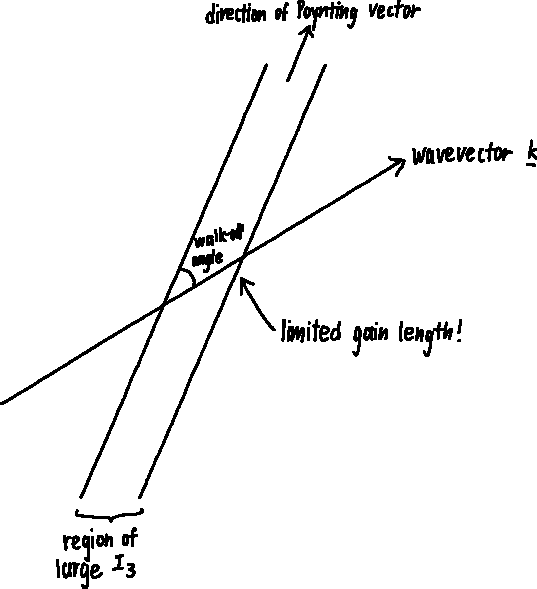
\includegraphics[width=.6\linewidth]{q2-walk-off}
	\end{figure}
	
	However by periodically reversing the axes in a poled crystal, we may reverse the walk-off periodically and keep the deviation minimal -- thereby increasing the useful gain length of the crystal.
\end{parts}